\documentclass[11pt]{amsart}


\usepackage{geometry}                % See geometry.pdf to learn the layout options. There are lots.
\geometry{a4paper}                   % ... or a4paper or a5paper or ...
%\geometry{landscape}                % Activate for for rotated page geometry
\usepackage[parfill]{parskip}    % Activate to begin paragraphs with an empty line rather than an indent
\usepackage{enumitem}
\usepackage{graphicx}
\usepackage{amssymb}
\usepackage{amsmath}
\usepackage{cancel}
\usepackage{epstopdf}
\DeclareGraphicsRule{.tif}{png}{.png}{`convert #1 `dirname #1`/`basename #1 .tif`.png}
\usepackage{breqn}
\usepackage{float}

\title{Econ 210C Problem Set \# 2}
\author{Minki Kim}
%\date{}                                           % Activate to display a given date or no date

\begin{document}




\maketitle

\section{Investment and the Housing Market}
\subsection{Explain the model}
\begin{enumerate}
	\item $I = \psi (P)$: Gross investment in housing is an increasing function of the price of houses. This specification makes sense because housing investment is interpreted as housing supply. 
	\item $r + \delta = (R + \dot{P})/P$: I assume that $\delta$ denotes the depreciation rate of a house. LHS is opportunity costs of investing into a house: forgone real interest rate and depreciation of the house. RHS is benefits of investing into a house: (real) rental payment and capital gains from the price of house. 
	\item $R = R(H)$: Rental cost $R$ is a decreasing function of available quantity of housing stock. 
	\item $\dot{H} = I - \delta H$: Change in $H$ is the difference between housing investment (new housing) and depreciated housing stock. 
\end{enumerate}
The model is closed: it has 4 endogenous variables ($I,R,P,H$) with 4 equations.

\subsection{Reduce the model into a 2-equation system}
\begin{align*}
\dot{H} &= \psi(P) - \delta H \\
r + \delta &= (R(H) + \dot{P}) / P
\end{align*}
Here $R$ is a function, not a variable. 
\subsection{Draw phase diagram}
*Lines do not have to be linear. 
\begin{figure}[H]
	\centering
	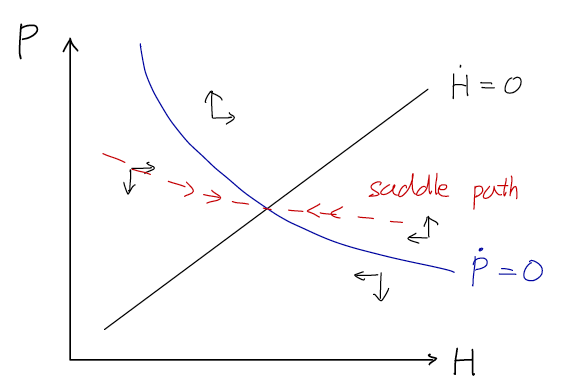
\includegraphics[width=0.65\textwidth]{1c_Minki.png}
\end{figure}

\subsection{Steady state effect of an increase in the real interest rate}
$r$ only shows up in the equation for $\dot{P}$. Rewriting the equation: 
\begin{equation*}
\dot{P} + R(H) = P (r + \delta)
\end{equation*}
Given a level of $P$, an increase in $r$ makes RHS larger, requiring $R(H)$ getting larger by the same amount to satisfy $\dot{P} = 0$. Since $R$ is a decreasing function of $H$, it means that $H$ has to decrease. Hence, $\dot{P} = 0$ locus shifts to the left. 

\subsection{Permanent increase in the real interest rate} Suppose the real interest rate changes from $r$ to $r^{*}$, where $r < r^{*}$. Recall that in the initial steady state, $P = \frac{R(H)}{r+\delta}$. At the arrival of the change, $P$ drops to the level $\frac{R(H)}{r^{*} + \delta}$. Cheaper real price of housing assets (or higher opportunity cost of investing in housing) reduces the amount of housing investments. As the housing investment decreases, the quantity of housing stock gradually decreases, until $R(H)$ goes up enough to satisfy $\dot{P}=0$ again.   
\begin{figure}[H]
	\centering
	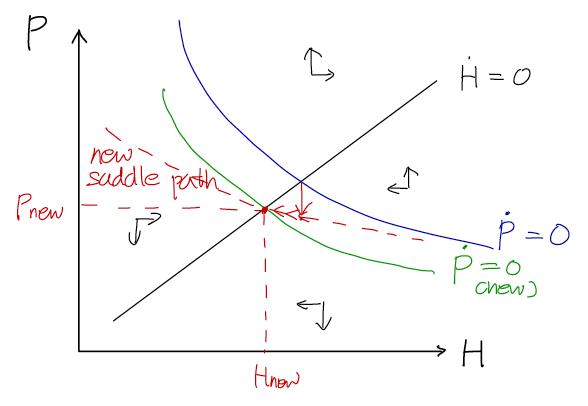
\includegraphics[width=0.65\textwidth]{1e1_Minki.png}
\end{figure}
Below is the impulse responses of each variable in response to the interest rate change. 
\begin{figure}[H]
	\centering
	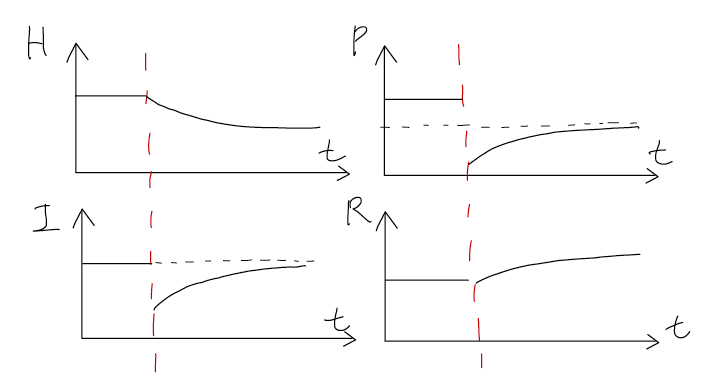
\includegraphics[width=0.7\textwidth]{1e2_Minki.png}
\end{figure}

\section{Discount Factor Shock}
\section{News Shock}
\section{Labor Supply}
\section{Impulse Responses}
\section{Impulse Responses (2)}



\end{document}
